
\section{Overview}
\label{sec:overview}

\begin{figure}[!t]
  \centering
  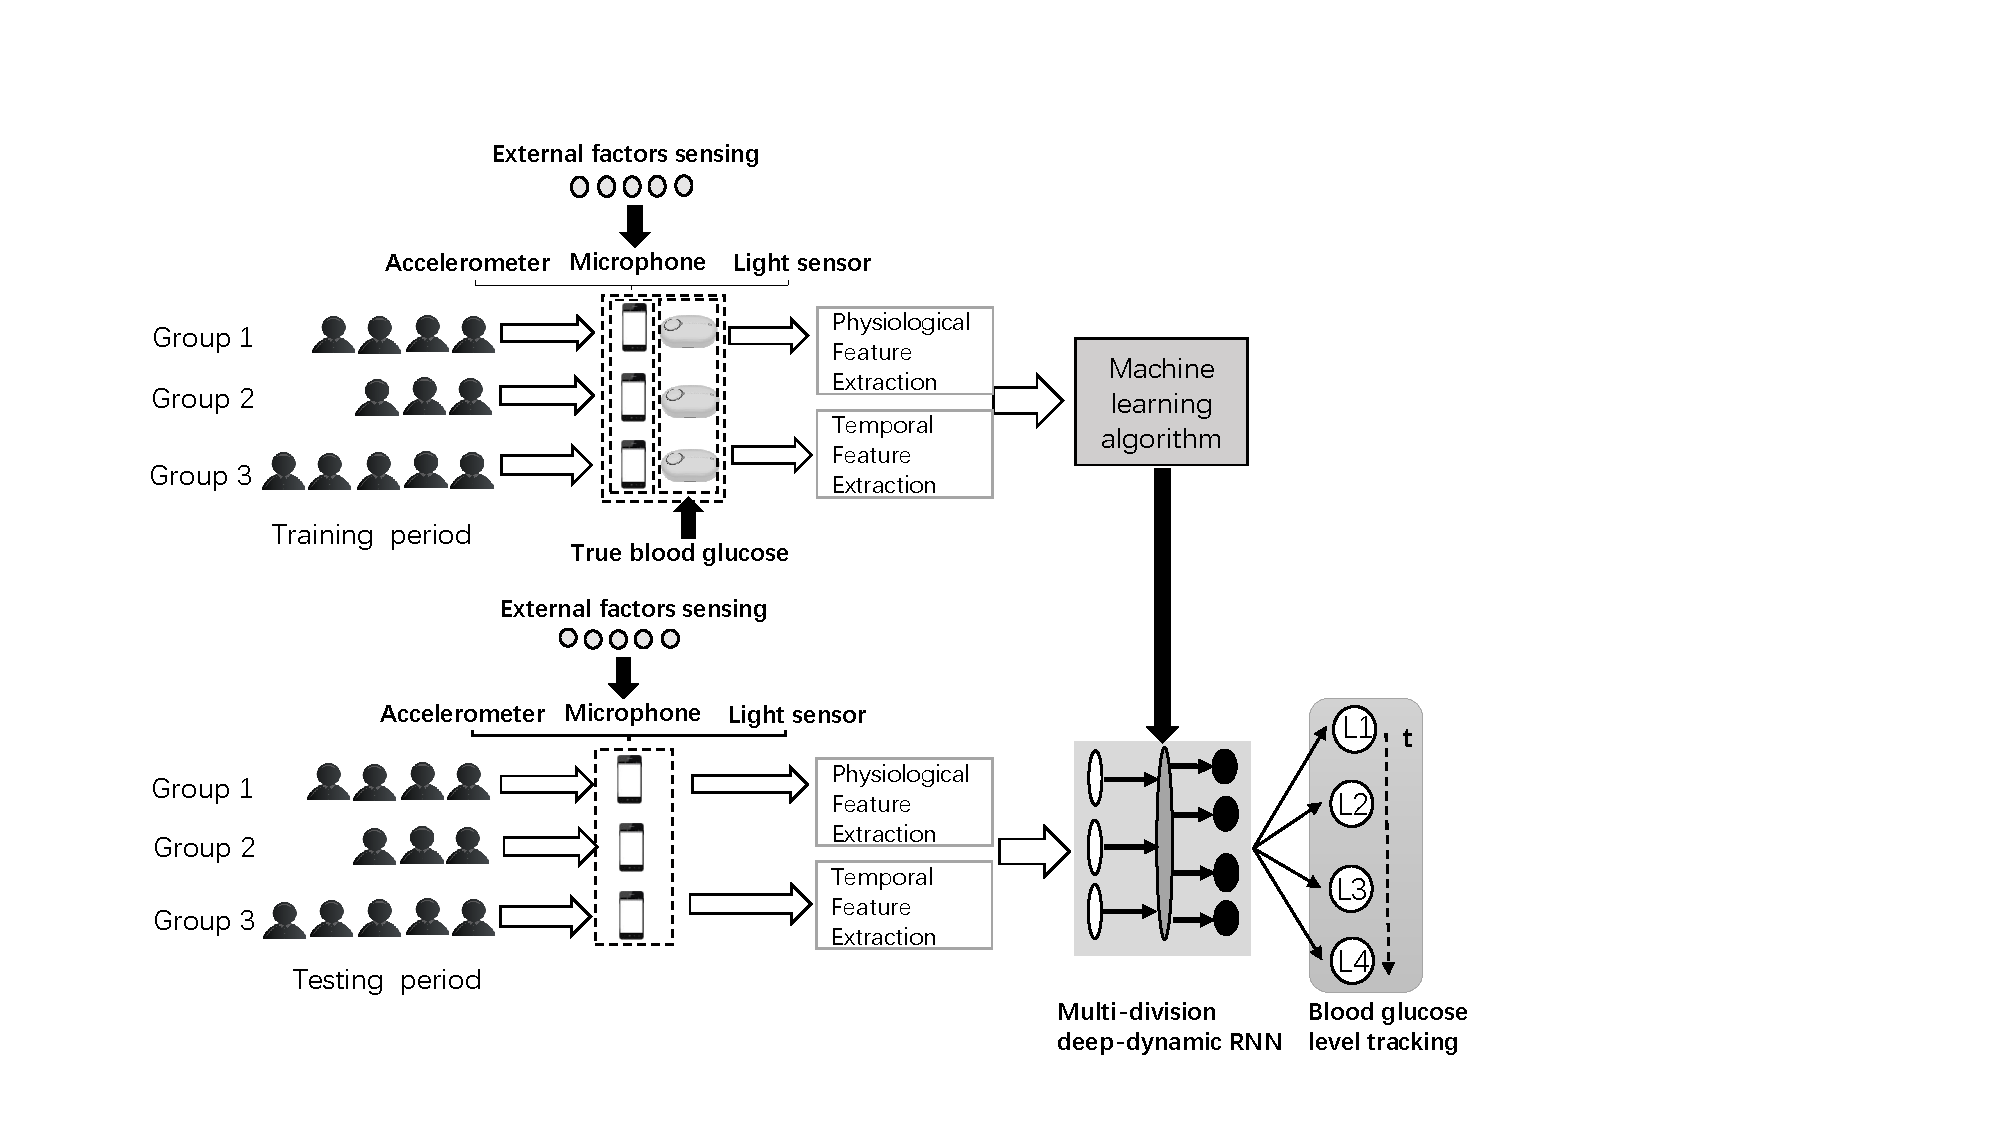
\includegraphics[width=1\columnwidth]{./img/System_Arch.pdf}
  \caption{The system architecture}
  \label{fig:architecture}
\end{figure}



The framework of \sysname is composed of three major components: external factor collection module, multi-task deep RNN module and blood glucose level tracking module. 

In the external factors collection module, the users are required to recrd their information into application, including of the diabetes type, drug, insulin and food intake. Meanwhile, \sysname triggers the embedded sensors to sense the physical activities and sleep quality of user.
\sysname classifies the users into three groups based on glucose types afterwards.
In the multi-task deep RNN (\modelname) model, the feature representation is firstly learnt within the users in a same group. Then, a deep RNN layer is trained based on the dataset of all users, which is to establish the dynamic relationships between the outer contextual factors and the corresponding blood glucose level. In the last, \modelname learns the personality of each user by the personality layer.
Based on the results of \modelname model, \sysname tracks the current blood glucose level in the last module. Once \sysname detects the abnormal points of blood glucose ( \ie in a \emph{high} or \emph{low} blood glucose level ), it reminds the user to measure the blood glucose by a clinical CGM or finger pricking method for a double-check.






%The framework of \sysname is shown as \figref{fig:architecture}, consisting of four major components.
%The first one is the external factors collection.
%The users are required to enter their basic information into application, including of the age, the gender, the diabetes type and the year of diagnosis.

%After a user measures his/her blood glucose by a CGM, the records of the blood glucose along with the outer contextual factors occurred during the measurement are uploaded to an individual database automatically.
%Afterwards, a RNN model is trained based on the dataset to establish the relationships between the outer contextual factors and the corresponding blood glucose level.
%It then is fed into the user's smartphone.
%When the user does not wear the CGM, \sysname detects the outer contextual factors with embedded sensors in the smartphones, and infers the current blood glucose level based on the trained model.
%Once \sysname detects the abnormal points of blood glucose ( \ie in a \emph{high} or \emph{low} blood glucose level ), it reminds the user to measure the blood glucose by a clinical CGM for a further control.

The extraction mechanisms of outer contextual factors are detailed as follows.

\emph{Physical activity}:
\sysname leverages the accelerometer to detect the user's activities by the approaches in \cite{bayat2014study}, as well as the corresponding time costs.
\sysname then measures the calorie of user's physical consumption.

\emph{Food intake}:
\sysname measures the food's effect on a person's blood glucose level based on the glycemic index.

\emph{Clinical drug intake}:
\sysname records the name and amount of the drug that user eat.

\emph{Time}:
\sysname invokes the timer embedded in the smartphone to record the time.

\emph{Sleep quality}:
\sysname measures the user's sleep by the approach in \cite{gu2014intelligent}.
